\documentclass[a4paper,12pt]{article}

% Самые необходимые пакеты
\usepackage[T2A]{fontenc}
\usepackage[utf8]{inputenc}
\usepackage[russian]{babel}
\usepackage{geometry}
\usepackage{amsmath}
\usepackage{graphicx}
\usepackage{float} 
\usepackage{xcolor}
\usepackage{listings}
\usepackage{hyperref}
\usepackage{array}
\usepackage{caption}
\usepackage{booktabs}
\usepackage{amssymb}
\usepackage{caption}
\usepackage{subcaption}

\lstset{
	language=Matlab,
	basicstyle=\ttfamily\small,
	keywordstyle=\color{blue}\bfseries,
	commentstyle=\color{gray}\itshape,
	stringstyle=\color{red},
	numberstyle=\tiny\color{gray},
	numbers=left,
	stepnumber=1,
	numbersep=8pt,
	backgroundcolor=\color{white},
	frame=single,
	breaklines=true,
	breakatwhitespace=true,
	tabsize=4,
	showspaces=false,
	showstringspaces=false,
	captionpos=b,
	escapeinside={\%*}{*)}, % для вставки LaTeX кода внутри листинга
}
% Настройка геометрии
\geometry{left=1.5cm, right=2cm, bottom=2cm, top=2cm}

\begin{document}
	
	% Титульный лист
	\begin{titlepage}
		\centering
		\vspace*{1cm}
		
		% Министерство
		{\small
			Министерство науки и высшего образования Российской Федерации\\
			Федеральное государственное автономное образовательное учреждение\\
			высшего образования\\
			«Национальный исследовательский университет ИТМО»\\
		}
		
		\vspace{2cm}
		
		% Факультет
		{\large
			Факультет систем управления и робототехники\\
		}
		
		\vspace{3cm}
		
		% Основной заголовок
		{\Huge\bfseries
			ОТЧЕТ\\
		}
		\vspace{0.5cm}
		{\LARGE\bfseries
			о лабораторной работе №2\\
		}
		
		\vspace{1cm}
		
		% Дисциплина и тема
		{\Large
			По дисциплине: «Линейные системы автоматического управления»\\
			\vspace{0.5cm}
			Тема: «Свободное движение, устойчивость»\\
		}
		
		\vspace{3cm}
		
		% Информация о студенте и преподавателях
		\begin{minipage}{0.4\textwidth}
			\raggedright
			{\large
				Студент:\\
			}
			Охрименко Е. Д.\\
			Поток: 1.1.3\\
			Вариант: 17\\
		\end{minipage}
		\hfill
		\begin{minipage}{0.4\textwidth}
			\raggedleft
			{\large
				Преподаватель:\\
			}
			Пашенко А. В.\\
		\end{minipage}
		
		\vfill
		
		% Город и год
		{\large
			Санкт-Петербург\\
			2025\\
		}
		
	\end{titlepage}
	
	\newpage
	\tableofcontents
	\newpage
	
	\section{Задание. Свободное движение}
	
	В этом задании рассмотрю линейную систему второго порядка, описываемую дифференциальным уравнением:
	
	\[
		\ddot{y} + a_1 \dot{y} + a_0 y = a_0 u(t)
	\]
	
	Требуется:
	
	\begin{itemize}
		\item Построить структурную схему системы с использованием элементарных блоков. На схеме указать блоки, на которых задаются начальные условия \( y(0) \), \( \dot{y}(0) \).
		\item Для каждого из шести экспериментов определить коэффициенты \( a_1 \), \( a_0 \) по заданным значениям корней характеристического уравнения \( \lambda_1, \lambda_2 \).
		\item Получить аналитическое выражение свободной составляющей движения \( y_{\text{св}}(t) \) (при \( u(t) = 0 \)).
		\item Выполнить моделирование системы и сравнить численные и аналитические результаты.
		\item Проанализировать устойчивость системы на основе корней и графиков \( y_{\text{св}}(t) \).
	\end{itemize}
	
	\subsection{Аналитические расчеты}

	Общее уравнение:
	
	\[
	\ddot{y} + a_1 \dot{y} + a_0 y = a_0 u(t)
	\]
	
	Так как движение свободное, то \(u(t) = 0\):
	
	\[
	\ddot{y} + a_1 \dot{y} + a_0 y = 0
	\]
	
	Запишу хараетеристическое уравнение для этого дифференциального уравнения:
	
	\[
	\lambda^2 + a_1 \lambda + a_0 = 0
	\]
	
	Коэффициенты \(a_i\) могут быть найдены по теореме Виета:
	
	\[
		\begin{cases}
			a_1 = - (\lambda_1 + \lambda_2) \\
			a_0 = \lambda_1 \cdot \lambda_2
		\end{cases}
	\]
	
	Используя Таблицу 1 проведу расчеты для каждого эксперимента.
	
	\begin{table}[H]
		\centering
		\caption{Параметры экспериментов: 17 вариант}
		\label{tab:experiment_parameters}
		\renewcommand{\arraystretch}{1.3}
		\begin{tabular}{@{}ccllc@{}}
			\toprule
			№ эксперимента & Корень \(\lambda_1\) & Корень \(\lambda_2\) & \(y(0)\) & \(\dot{y}(0)\) \\
			\midrule
			1 & \(-6\) & \(-6.5\) & 1 & 0 \\
			2 & \(-2.9 + j7\) & \(-2.9 - j7\) & 1 & 0 \\
			3 & \(j19\) & \(-j19\) & 1 & 0 \\
			4 & \(0.9 + j7\) & \(0.9 - j7\) & 0.05 & 0 \\
			5 & \(6\) & \(6.5\) & 0.05 & 0 \\
			6 & \(-1.8\) & \(1.8\) & 0 & 0.1 \\
			\bottomrule
		\end{tabular}
	\end{table}
	
	
	\begin{itemize}
		
		\item Эксперимент 1

		Найду коэффициенты \(a_i\):
		
		\[
		\begin{cases}
			a_1 = -(\lambda_1 + \lambda_2) = -(-6 - 6.5) = 12.5 \\[8pt]
			a_0 = \lambda_1 \cdot \lambda_2 = (-6)(-6.5) = 39
		\end{cases}
		\]
		
		Дифференциальное уравнение системы имеет вид:
		\[
		\ddot{y} + 12.5 \dot{y} + 39 y = 0
		\]
		
		Корни — действительные и различные, значит общее решение:
		\[
		y(t) = C_1 e^{-6t} + C_2 e^{-6.5t}
		\]
		
		Возьму производную:
		
		\[
		\dot{y}(t) = -6 C_1 e^{-6t} - 6.5 C_2 e^{-6.5t}
		\]
		
		Подставлю начальные условия (\( t=0 \)):
		\[
		\begin{cases}
		y(0) = C_1 + C_2 = 1 \\[8pt]
		\dot{y}(0) = -6 C_1 - 6.5 C_2 = 0
		\end{cases} \Rightarrow \quad
		\begin{cases}
			C_1 = 13 \\[8pt]
			C_2 = -12
		\end{cases}		
		\]
		
		Итоговое уравнение:
		
		\[
			y(t) = 13 e^{-6t} - 12 e^{-6.5t}
		\]
		
		\item Эксперимент 2
		
		Найду коэффициенты \(a_i\):
		
		\[
		\begin{cases}
			a_1 = -(\lambda_3 + \lambda_4) = -\big((-2.9 + j7) + (-2.9 - j7)\big) = -(-5.8) = 5.8 \\[8pt]
			a_0 = \lambda_3 \cdot \lambda_4 = (-2.9 + j7)(-2.9 - j7) = (-2.9)^2 + 7^2 = 8.41 + 49 = 57.41
		\end{cases}
		\]
		
		Дифференциальное уравнение системы:
		
		\[
		\ddot{y} + 5.8 \dot{y} + 57.41 y = 0
		\]
		
		Корни — комплексно-сопряжённые, значит решение имеет вид:
		
		\[
		y(t) = e^{-2.9 t} \left( C_1 \cos 7 t + C_2 \sin 7 t \right)
		\]
		
		Возьму производную:
		
		\[
		\dot{y}(t) = e^{-2.9 t} \left[ (C_1 \cos 7 t + C_2 \sin 7 t)(-2.9) + (-7 C_1 \sin 7 t + 7 C_2 \cos 7 t) \right]
		\]
		
		
		Подставлю начальные условия при \(t=0\):
		
		\[
		\begin{cases}
			y(0) = C_1 = 1 \\[8pt]
			\dot{y}(0) = -2.9 \cdot C_1 + 7 \cdot C_2 = 0
		\end{cases}
		\quad \Rightarrow \quad
		\begin{cases}
			C_1 = 1 \\[8pt]
			C_2 = \dfrac{29}{70}
		\end{cases}
		\]
		
		
		
		Итоговое решение:
		
		\[
			y(t) = e^{-2.9 t} \left( \cos 7 t + \frac{29}{70} \sin 7 t \right)
		\]
		
		\item Эксперимент 3
		
		Найду коэффициенты \(a_i\):
		
		\[
		\begin{cases}
			a_1 = -(\lambda_5 + \lambda_6) = -(j19 + (-j19)) = -0 = 0 \\[8pt]
			a_0 = \lambda_5 \cdot \lambda_6 = j19 \cdot (-j19) = -(j)^2 \cdot 19^2 = 19^2 = 361
		\end{cases}
		\]
		
		Дифференциальное уравнение системы:

		\[
		\ddot{y} + 361 y = 0
		\]
		
		Корни — чисто мнимые, значит решение имеет вид:
		
		\[
		y(t) = C_1 \cos 19 t + C_2 \sin 19 t
		\]
		
		Возьму производную:
		
		\[
		\dot{y}(t) = -19 C_1 \sin 19 t + 19 C_2 \cos 19 t
		\]
		
		Подставлю начальные условия при \(t=0\):
		
		\[
		\begin{cases}
			y(0) = C_1 = 1 \\[8pt]
			\dot{y}(0) = 19 C_2 = 0
		\end{cases}
		\quad \Rightarrow \quad
		\begin{cases}
			C_1 = 1 \\[8pt]
			C_2 = 0.
		\end{cases}
		\]
		
		Итоговое решение:
		
		\[
			y(t) = \cos 19 t
		\]
		
		
		\item Эксперимент 4
		
		Найду коэффициенты \(a_i\):
		
		\[
		\begin{cases}
			a_1 = -(\lambda_7 + \lambda_8) = -\big((0.9 + j7) + (0.9 - j7)\big) = -(1.8) = -1.8 \\[8pt]
			a_0 = \lambda_7 \cdot \lambda_8 = (0.9 + j7)(0.9 - j7) = 0.9^2 + 7^2 = 0.81 + 49 = 49.81
		\end{cases}
		\]
		
		Дифференциальное уравнение системы:
		
		\[
		\ddot{y} - 1.8 \dot{y} + 49.81 y = 0
		\]
		
		Корни — комплексно-сопряжённые, значит решение имеет вид:
		
		\[
		y(t) = e^{0.9 t} \bigl( C_1 \cos 7 t + C_2 \sin 7 t \bigr)
		\]
		
		Возьму производную:
		
		\[
		\dot{y}(t) = e^{0.9 t} \bigl[ (C_1 \cos 7 t + C_2 \sin 7 t) \cdot 0.9 + (-7 C_1 \sin 7 t + 7 C_2 \cos 7 t) \bigr]
		\]
		
		Подставлю начальные условия при \( t = 0 \):
		
		\[
		\begin{cases}
			y(0) = C_1 = 0.05 \\[8pt]
			\dot{y}(0) = 0.9 C_1 + 7 C_2 = 0
		\end{cases}
		\quad \Rightarrow \quad
		\begin{cases}
			C_1 = 0.05 \\[8pt]
			C_2 = \dfrac{45}{7000}
		\end{cases}
		\]
		
		
		Итоговое решение:
		
		\[
		y(t) = e^{0.9 t} \left( 0.05 \cos 7 t - \dfrac{45}{7000} \sin 7 t \right)
		\]
		
		\item Эксперимент 5
		
		Найду коэффициенты \(a_i\):
		
		\[
		\begin{cases}
			a_1 = -(\lambda_9 + \lambda_{10}) = -(6 + 6.5) = -12.5 \\[8pt]
			a_0 = \lambda_9 \cdot \lambda_{10} = 6 \cdot 6.5 = 39
		\end{cases}
		\]
		
		Дифференциальное уравнение системы:
		
		\[
		\ddot{y} - 12.5 \dot{y} + 39 y = 0
		\]
		
		Корни — действительные и различные, значит решение имеет вид:
		
		\[
		y(t) = C_1 e^{6 t} + C_2 e^{6.5 t}
		\]
		
		Возьму производную:
		
		\[
		\dot{y}(t) = 6 C_1 e^{6 t} + 6.5 C_2 e^{6.5 t}
		\]
		
		Подставлю начальные условия при \(t = 0\):
		
		\[
		\begin{cases}
			y(0) = C_1 + C_2 = 0.05 \\[8pt]
			\dot{y}(0) = 6 C_1 + 6.5 C_2 = 0
		\end{cases} \Rightarrow \quad
		\begin{cases}
			C_1 = 0.65 \\[8pt]
			C_2 = -0.6
		\end{cases} 		
		\]
		
		Итоговое решение:
		
		\[
		y(t) = 0.65 e^{6 t} - 0.6 e^{6.5 t}
		\]
		
		
		\item Эксперимент 6
		
		Найду коэффициенты \(a_i\):
		
		\[
		\begin{cases}
			a_1 = -(\lambda_{11} + \lambda_{12}) = -(-1.8 + 1.8) = -0 = 0 \\[8pt]
			a_0 = \lambda_{11} \cdot \lambda_{12} = (-1.8)(1.8) = -3.24
		\end{cases}
		\]
		
		Дифференциальное уравнение системы:

		\[
		\ddot{y} - 3.24 y = 0.
		\]
		
		Корни — действительные и разные:
		
		\[
		\lambda = \pm \sqrt{3.24} = \pm 1.8.
		\]
		
		Общее решение:
		
		\[
		y(t) = C_1 e^{1.8 t} + C_2 e^{-1.8 t}.
		\]
		
		Возьму производную:
		
		\[
		\dot{y}(t) = 1.8 C_1 e^{1.8 t} - 1.8 C_2 e^{-1.8 t}.
		\]
		
		Подставлю начальные условия при \(t=0\):
		
		\[
		\begin{cases}
			y(0) = C_1 + C_2 = 0 \\[8pt]
			\dot{y}(0) = 1.8 C_1 - 1.8 C_2 = 0.1
		\end{cases} \Rightarrow \quad
		\begin{cases}
		C_1 = \dfrac{1}{36} \\[8pt]
		C_2 = -\dfrac{1}{36}
		\end{cases} 
		\]
		
		Итоговое решение:
		
		\[
		y(t) = \frac{1}{36} e^{1.8 t} - \frac{1}{36} e^{-1.8 t}.
		\]
		
			
		\end{itemize}
		
		\subsection{Структурная схема системы}
		
		Соберу схему для уравнения: \(
		\ddot{y} + a_1 \dot{y} + a_0 y = 0 \quad \Rightarrow \quad \ddot{y} = - a_1 \dot{y} - a_0 y
		\)
		
		\begin{figure}[H]
			\centering
			
\includegraphics[width=0.7\textwidth]{../images/task1/model1.png}
			\caption{Структурная схема системы}
		\end{figure}
		
		В блоках \texttt{Integrator} устанавлю параметры в поле \texttt{Initial condition}, которые соответствуют начальным условиям \(y(0)\) и \(\dot{y}(0)\) для каждого эксперимента.
		
		\subsection{Графики выходов}
		
		На графиках показано, как меняется выходной сигнал \(y(t)\) со временем для разных значений коэффициентов и начальных условий. На каждом графике видно, как система ведет себя — затухают колебания, колеблется с постоянной амплитудой или амплитуда растет. Значения по оси \(Time\) я подобрала так, чтобы поведение системы было хорошо заметно и наглядно.
		\[\]
		- В первом эксперименте корни характеристического уравнения: \[\forall i, \quad \lambda_i < 0, \quad \lambda_i \in \mathbb{R}
		\] Поэтому система будет асимптотически устойчивой. Это совпадает с поведением системы на графике.
		
		\begin{figure}[H]
			\centering
			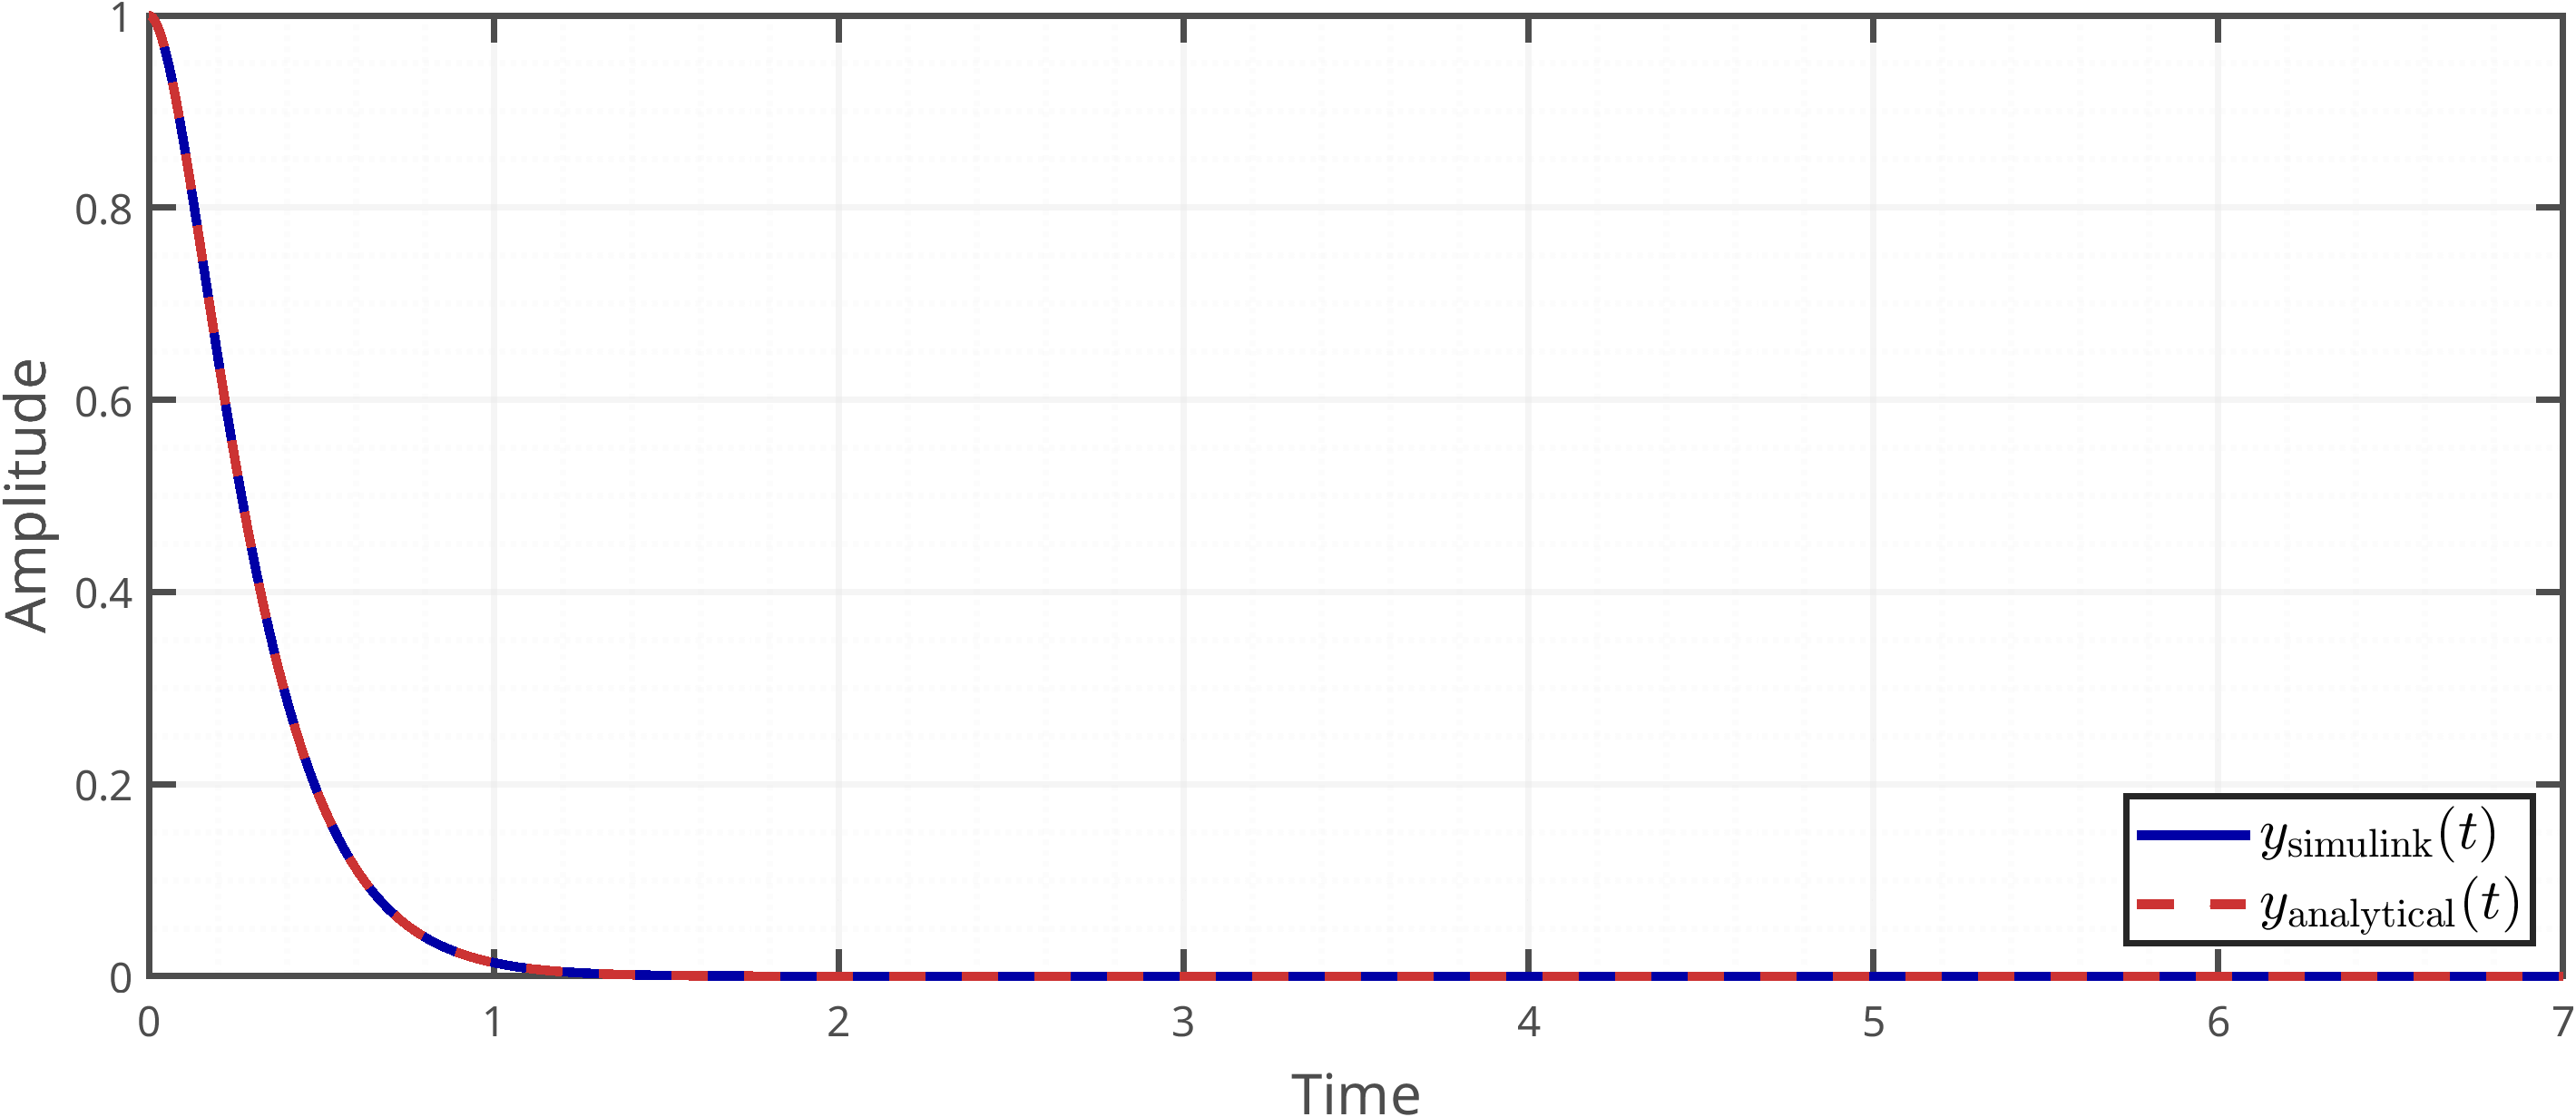
\includegraphics[width=1\textwidth]{../images/task1/y1.png}
			\caption{График эксперимента 1}
		\end{figure}
		\[\]
		
		Во втором эксперименте корни характеристического уравнения: \[\forall i, \quad \lambda_i < 0, \quad \lambda_i \in \mathbb{R}
		\] Поэтому система асимптотически устойчива. Это подтверждается поведением системы на графике.
		
		\begin{figure}[H]
			\centering
			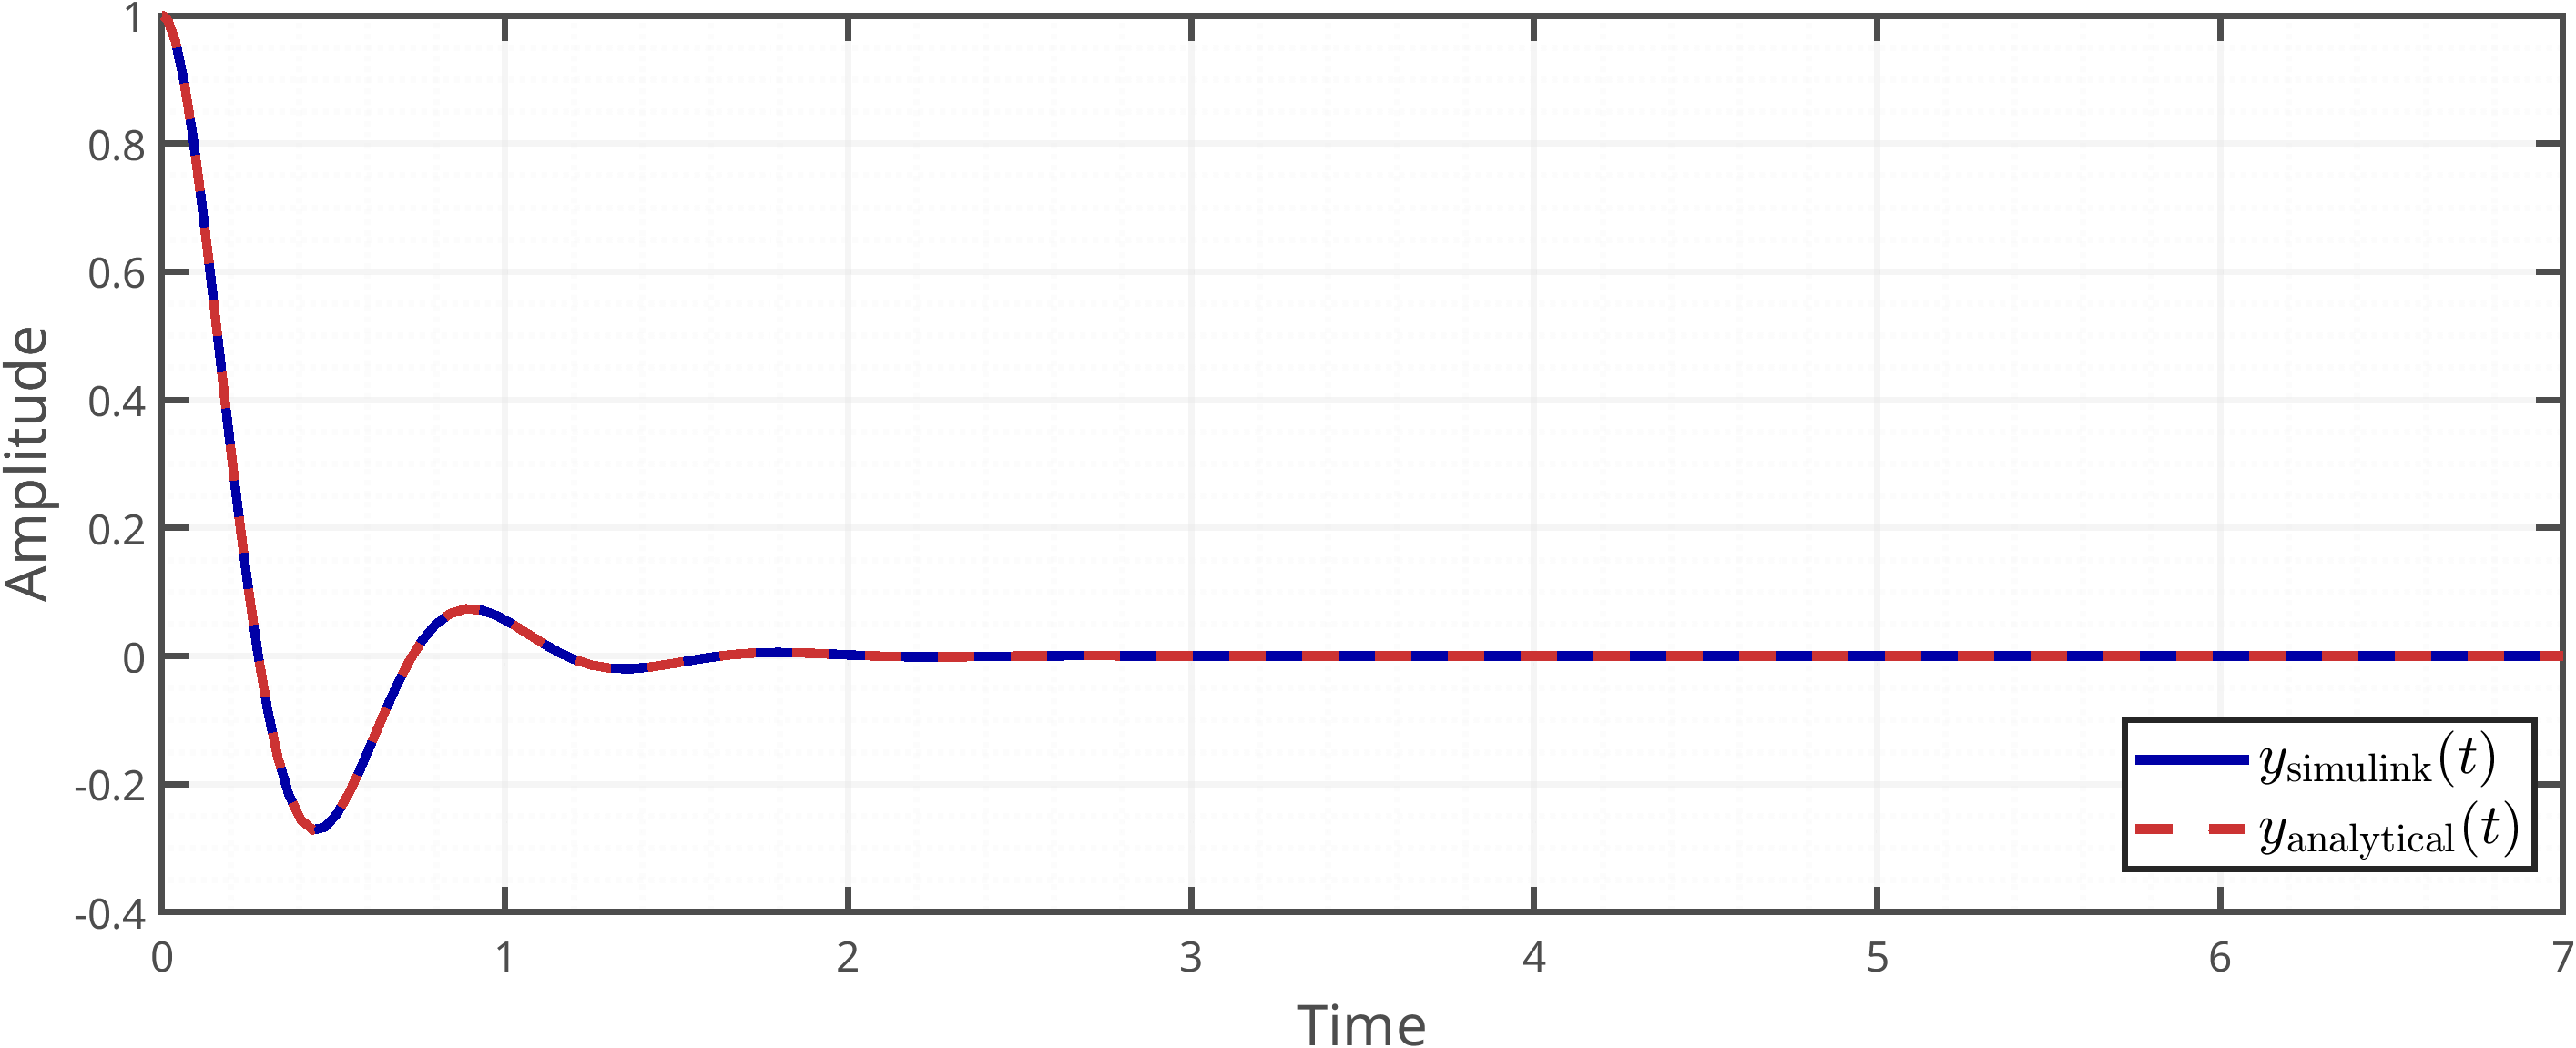
\includegraphics[width=1\textwidth]{../images/task1/y2.png}
			\caption{График эксперимента 2}
		\end{figure}
		\[\]
		В третьем эксперименте корни характеристического уравнения чисто мнимые:
		\[
		\forall i, \quad \operatorname{Re}(\lambda_i) = 0, \quad \lambda_i \in i\mathbb{R}
		\]
		Поэтому система устойчива. На графике это видно в виде колебаний с постоянной амплитудой.
		
		\begin{figure}[H]
			\centering
			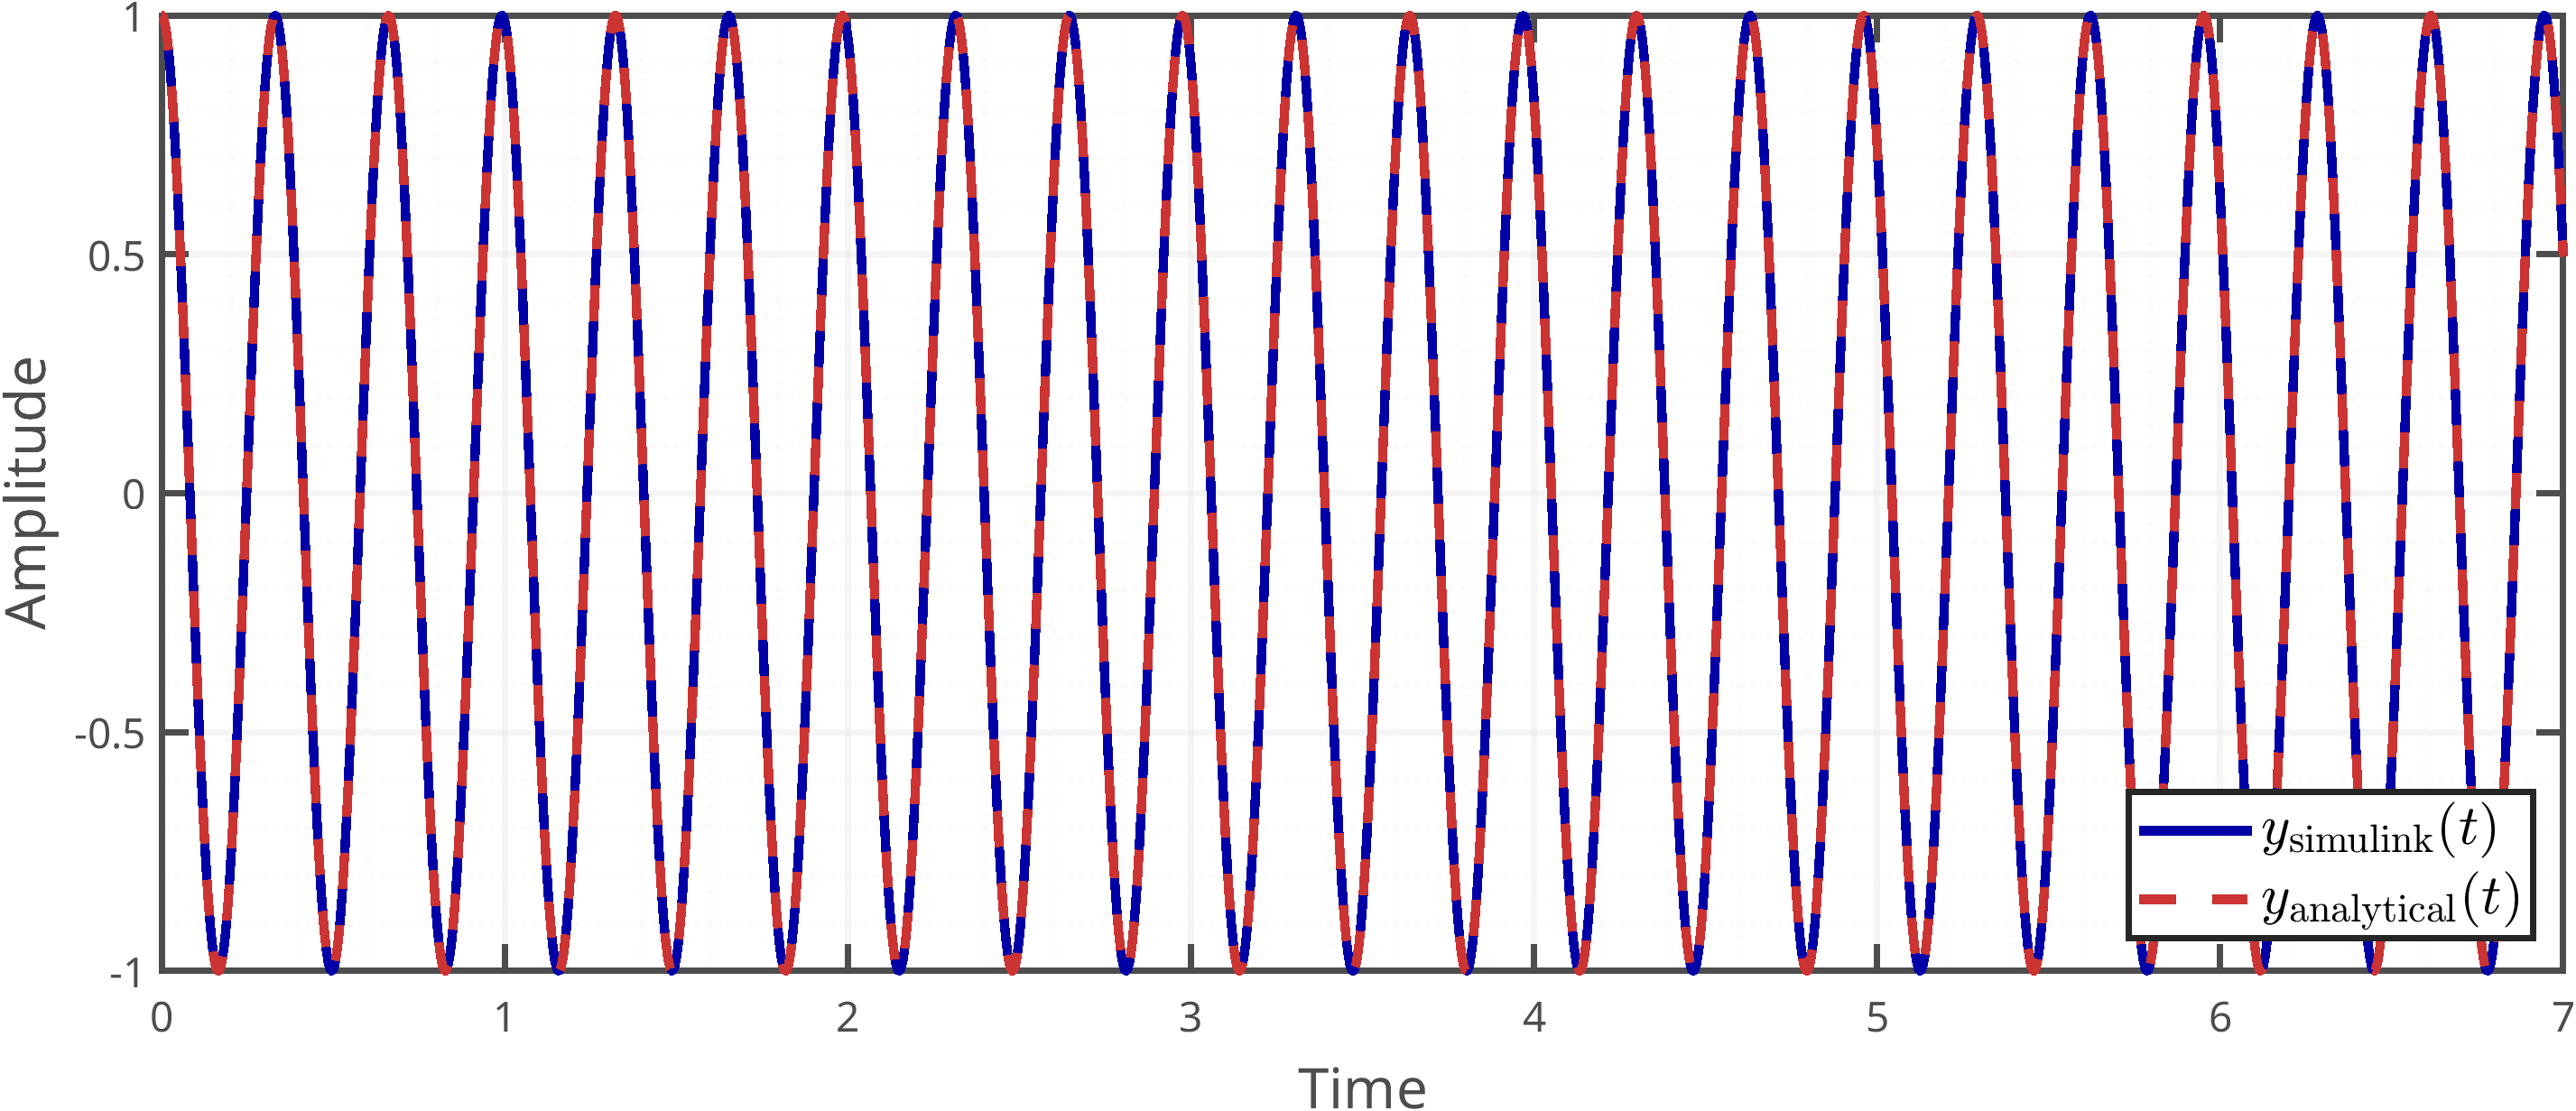
\includegraphics[width=1\textwidth]{../images/task1/y3.png}
			\caption{График эксперимента 3}
		\end{figure}
		\[\]
		В четвёртом эксперименте корни характеристического уравнения:
		\[
		\exists i: \quad \operatorname{Re}(\lambda_i) > 0, \quad \lambda_i \in \mathbb{C}
		\]
		Поэтому система неустойчива, что совпадает с ростом амплитуды колебаний на графике.
		
		\begin{figure}[H]
			\centering
			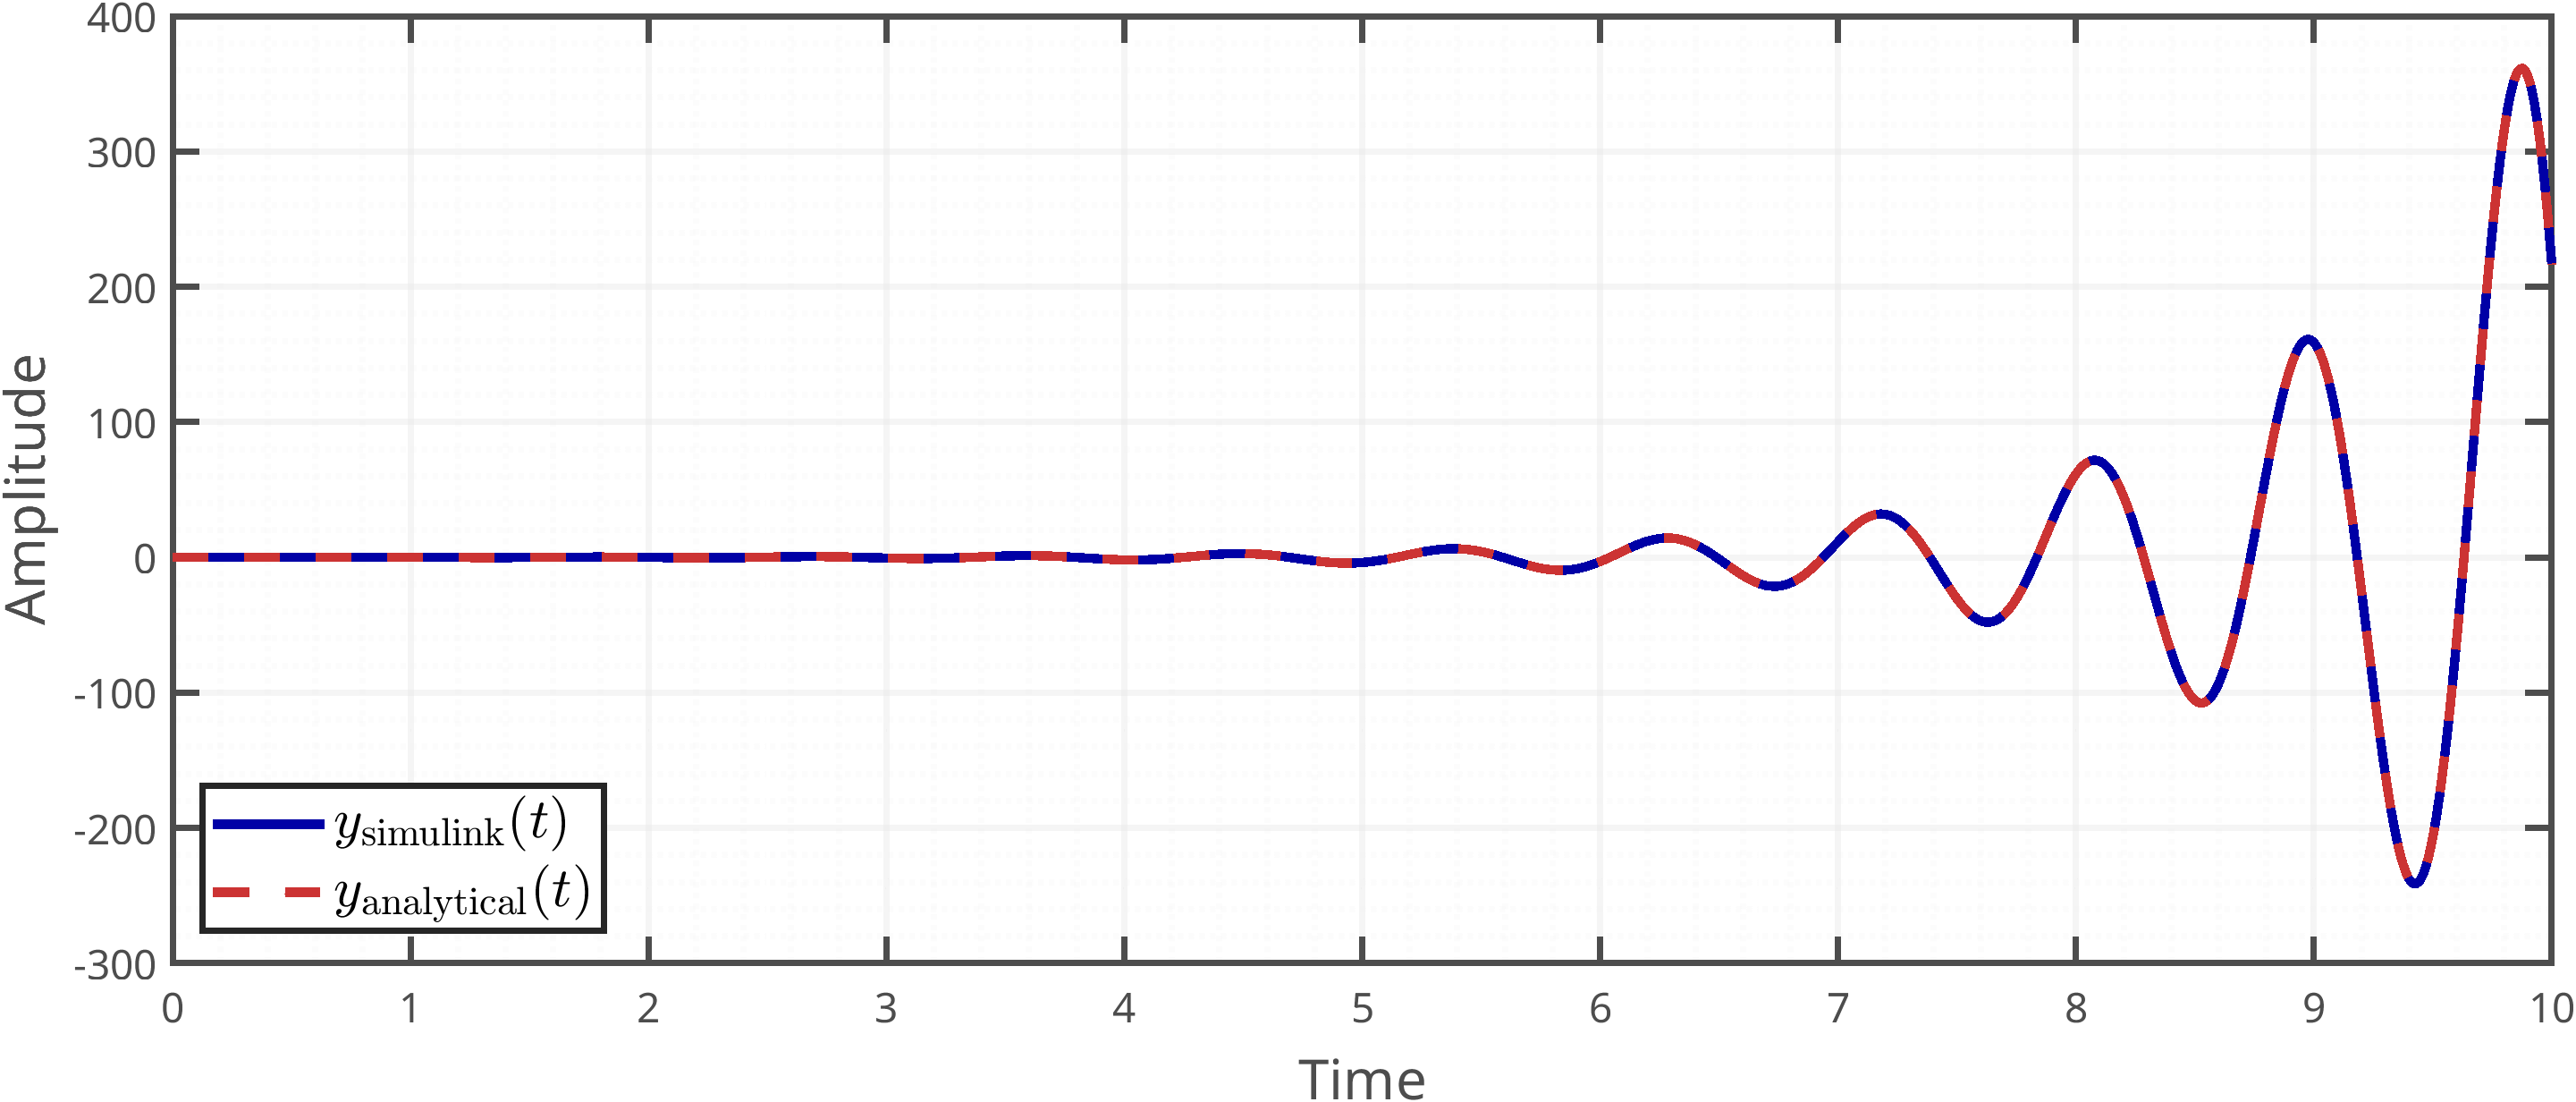
\includegraphics[width=1\textwidth]{../images/task1/y4.png}
			\caption{График эксперимента 4}
		\end{figure}
		\[\]
		В пятом эксперименте корни характеристического уравнения:
		\[
		\forall i, \quad \lambda_i > 0, \quad \lambda_i \in \mathbb{R}
		\]
		Система неустойчива.
		\begin{figure}[H]
			\centering
			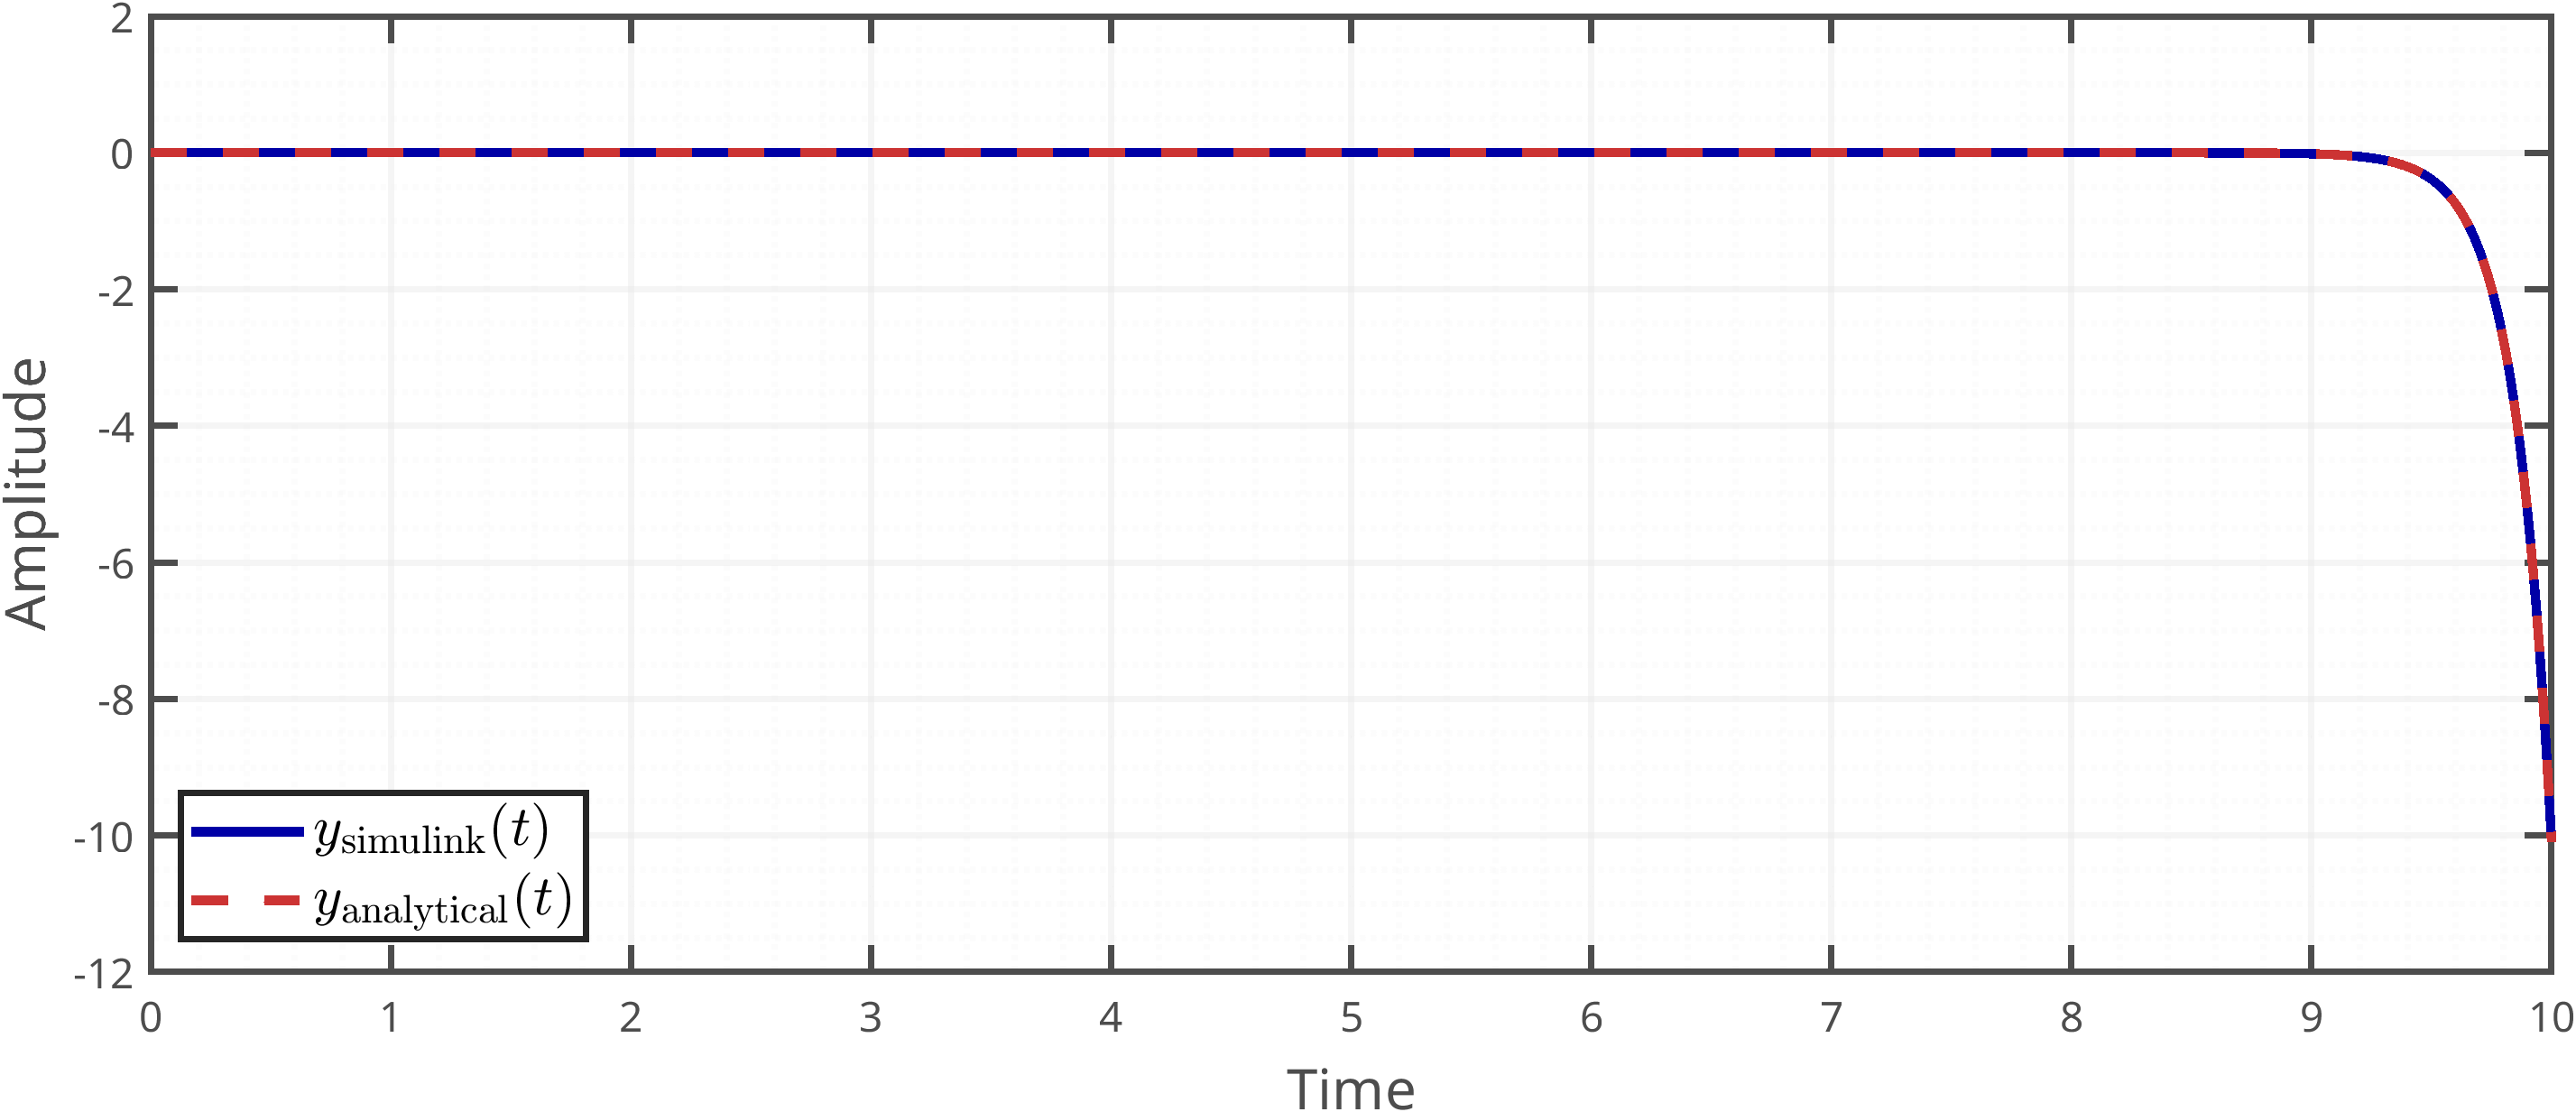
\includegraphics[width=1\textwidth]{../images/task1/y5.png}
			\caption{График эксперимента 5}
		\end{figure}
		\[\]
		В шестом эксперименте корни характеристического уравнения:
		\[
		\exists i: \quad \lambda_i > 0, \quad \exists j: \quad \lambda_j < 0, \quad \lambda_i, \lambda_j \in \mathbb{R}
		\]
		Поэтому система неустойчива из-за положительного корня.
		
		\begin{figure}[H]
			\centering
			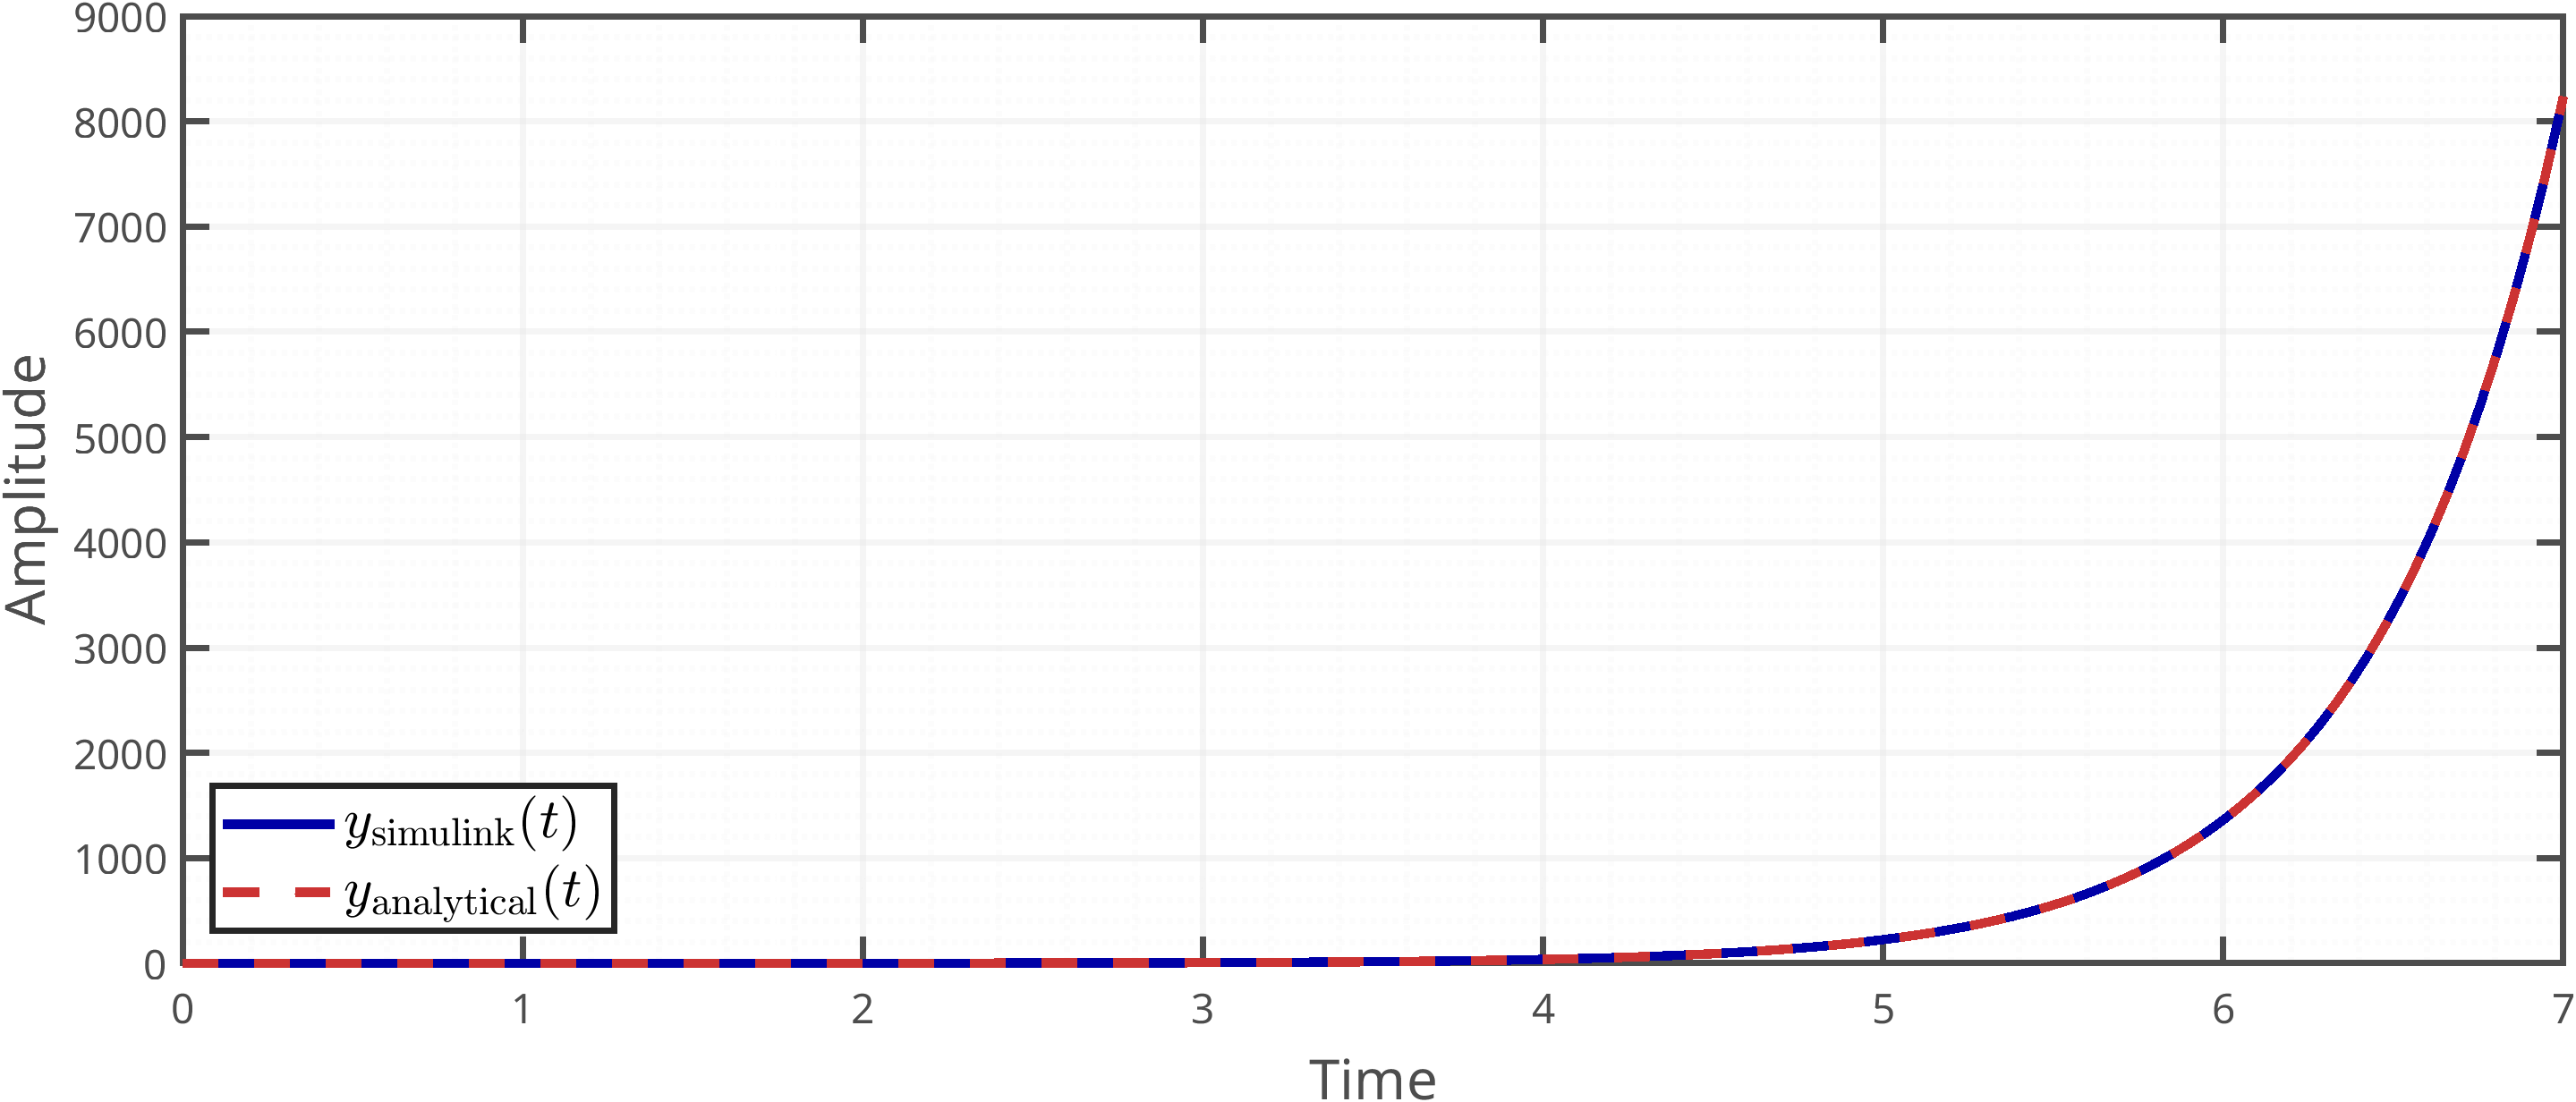
\includegraphics[width=1\textwidth]{../images/task1/y6.png}
			\caption{График эксперимента 6}
		\end{figure}
		
		
		\textbf{Итог: } Графики показывают, что при отрицательных вещественных корнях система затухает экспоненциально, при комплексных с отрицательной частью — затухающие колебания, при чисто мнимых — устойчивые колебания с постоянной амплитудой, а при положительной вещественной части — выход растёт, что соответствует неустойчивости.
		
		
		
		
		
		\newpage
		\section{Задание. Область устойчивости}
		
		Рассмотреть систему третьего порядка, заданную структурной схемой. 
		
		\begin{figure}[H]
			\centering
			
\includegraphics[width=1\textwidth]{../images/task2/model.png}
			\caption{Структурная схема системы}
		\end{figure}
		
		Требуется:
		
		\begin{itemize}
			\item Определить значения постоянных времени \(T_1\) и \(T_2\), при которых полюса передаточной функции совпадают с корнями \(\lambda_1\) и \(\lambda_2\) из Задания 1.
			\item Аналитически найти границу устойчивости в пространстве параметров \(K\) и \(T_1\) при фиксированном \(T_2\), используя критерий Гурвица, и построить график \(K(T_1)\).
			\item Аналогично определить границу устойчивости для параметров \(K\) и \(T_2\) при фиксированном \(T_1\), построить график \(K(T_2)\).
			\item Провести моделирование системы для трёх наборов параметров, соответствующих устойчивой, критической и неустойчивой системам, при входном воздействии \(g(t) = 1\).
			\item Проанализировать полученные графики и сделать выводы.
		\end{itemize}
		\subsection{Аналитические расчеты}
		
	 	Возьму два собственных значения:
		
		\[
		\lambda_1 = -6, \quad \lambda_2 = -6.5
		\]
		
		Эти значения определяют, при каких значениях параметров система будет вести себя с заданной скоростью затухания. Если рассмотреть звенья с передаточной функцией вида:
		
		\[
		\frac{1}{T_1 s + 1}, \quad \frac{1}{T_2 s + 1}
		\]
		
		то их полюса находятся по формуле:
		
		\[
		s = -\frac{1}{T}
		\]
		
		Приравнивая \( s = \lambda \), получаем:
		
		\[
		T_1 = \frac{1}{6}, \quad T_2 = \frac{1}{6.5}\]
		
		Передаточная функция системы
		
		\[
		W(s) = \frac{K}{s (T_1 s + 1)(T_2 s + 1)}
		\]
		
		
		
		
		Характеристическое уравнение системы:
		
		\[
		(T_1 T_2 s^2 + (T_1 + T_2)s + 1)s + K = 0
		\Rightarrow T_1 T_2 s^3 + (T_1 + T_2) s^2 + s + K = 0
		\]
		
		
		Система будет устойчивой, если все коэффициенты характеристического уравнения положительны и выполнено дополнительное условие:
		
		\[
		a_3 s^3 + a_2 s^2 + a_1 s + a_0 = 0
		\]
		\[
		\begin{cases}
			a_3 = T_1 T_2 \\
			a_2 = T_1 + T_2 \\
			a_1 = 1 \\
			a_0 = K
		\end{cases}
		\]
		
		Для устойчивости по критерию Гурвица необходимо:
		
		\[
		\Delta_2 = a_2 a_1 - a_3 a_0 > 0
		\Rightarrow (T_1 + T_2) - T_1 T_2 \cdot K > 0
		\Rightarrow K < \frac{T_1 + T_2}{T_1 T_2}
		\]
		
		Это выражение задаёт границу устойчивости в виде неравенства.
		
		
		Подставлю найденные ранее значения:
		
		\[
		T_1 = \frac{1}{6}, \quad T_2 = \frac{1}{6.5}
		\]
		
		Выполню расчёты:
		
		\[
		T_1 + T_2 = \frac{1}{6} + \frac{1}{6.5} = \frac{12.5}{39}, \quad
		T_1 T_2 = \frac{1}{6} \cdot \frac{1}{6.5} = \frac{1}{39}
		\]
		
		Подставлю в формулу границы устойчивости:
		
		\[
		K = \frac{T_1 + T_2}{T_1 T_2} = \dfrac{\dfrac{12.5}{39}}{\dfrac{1}{39}} = 12.5
		\]
		
		\textbf{Итог: }
		
		\begin{itemize}
			\item Если $K < 12.5$, система является устойчивой.
			\item Если $K = 12.5$, система находится на границе устойчивости.
			\item Если $K > 12.5$, система становится неустойчивой.
		\end{itemize}
		
		\subsection{Графическое изображение границы устойчивости}
		
		На рисунках ниже показаны границы устойчивости системы в зависимости от параметров \(K\) и \(T_1\) или \(T_2\).  
		\begin{itemize}
			\item На левом графике видно, как меняется допустимое значение коэффициента усиления \(K\) при изменении \(T_1\) и фиксированном \(T_2\).
			\item На правом — зависимость \(K\) от \(T_2\) при фиксированном \(T_1\).
		\end{itemize}
		Эти графики помогают визуально определить область устойчивости системы и оценить, как изменение параметров влияет на устойчивость.
		
		\begin{figure}[htbp]
			\centering
			\begin{minipage}[b]{0.485\textwidth}
				\centering
				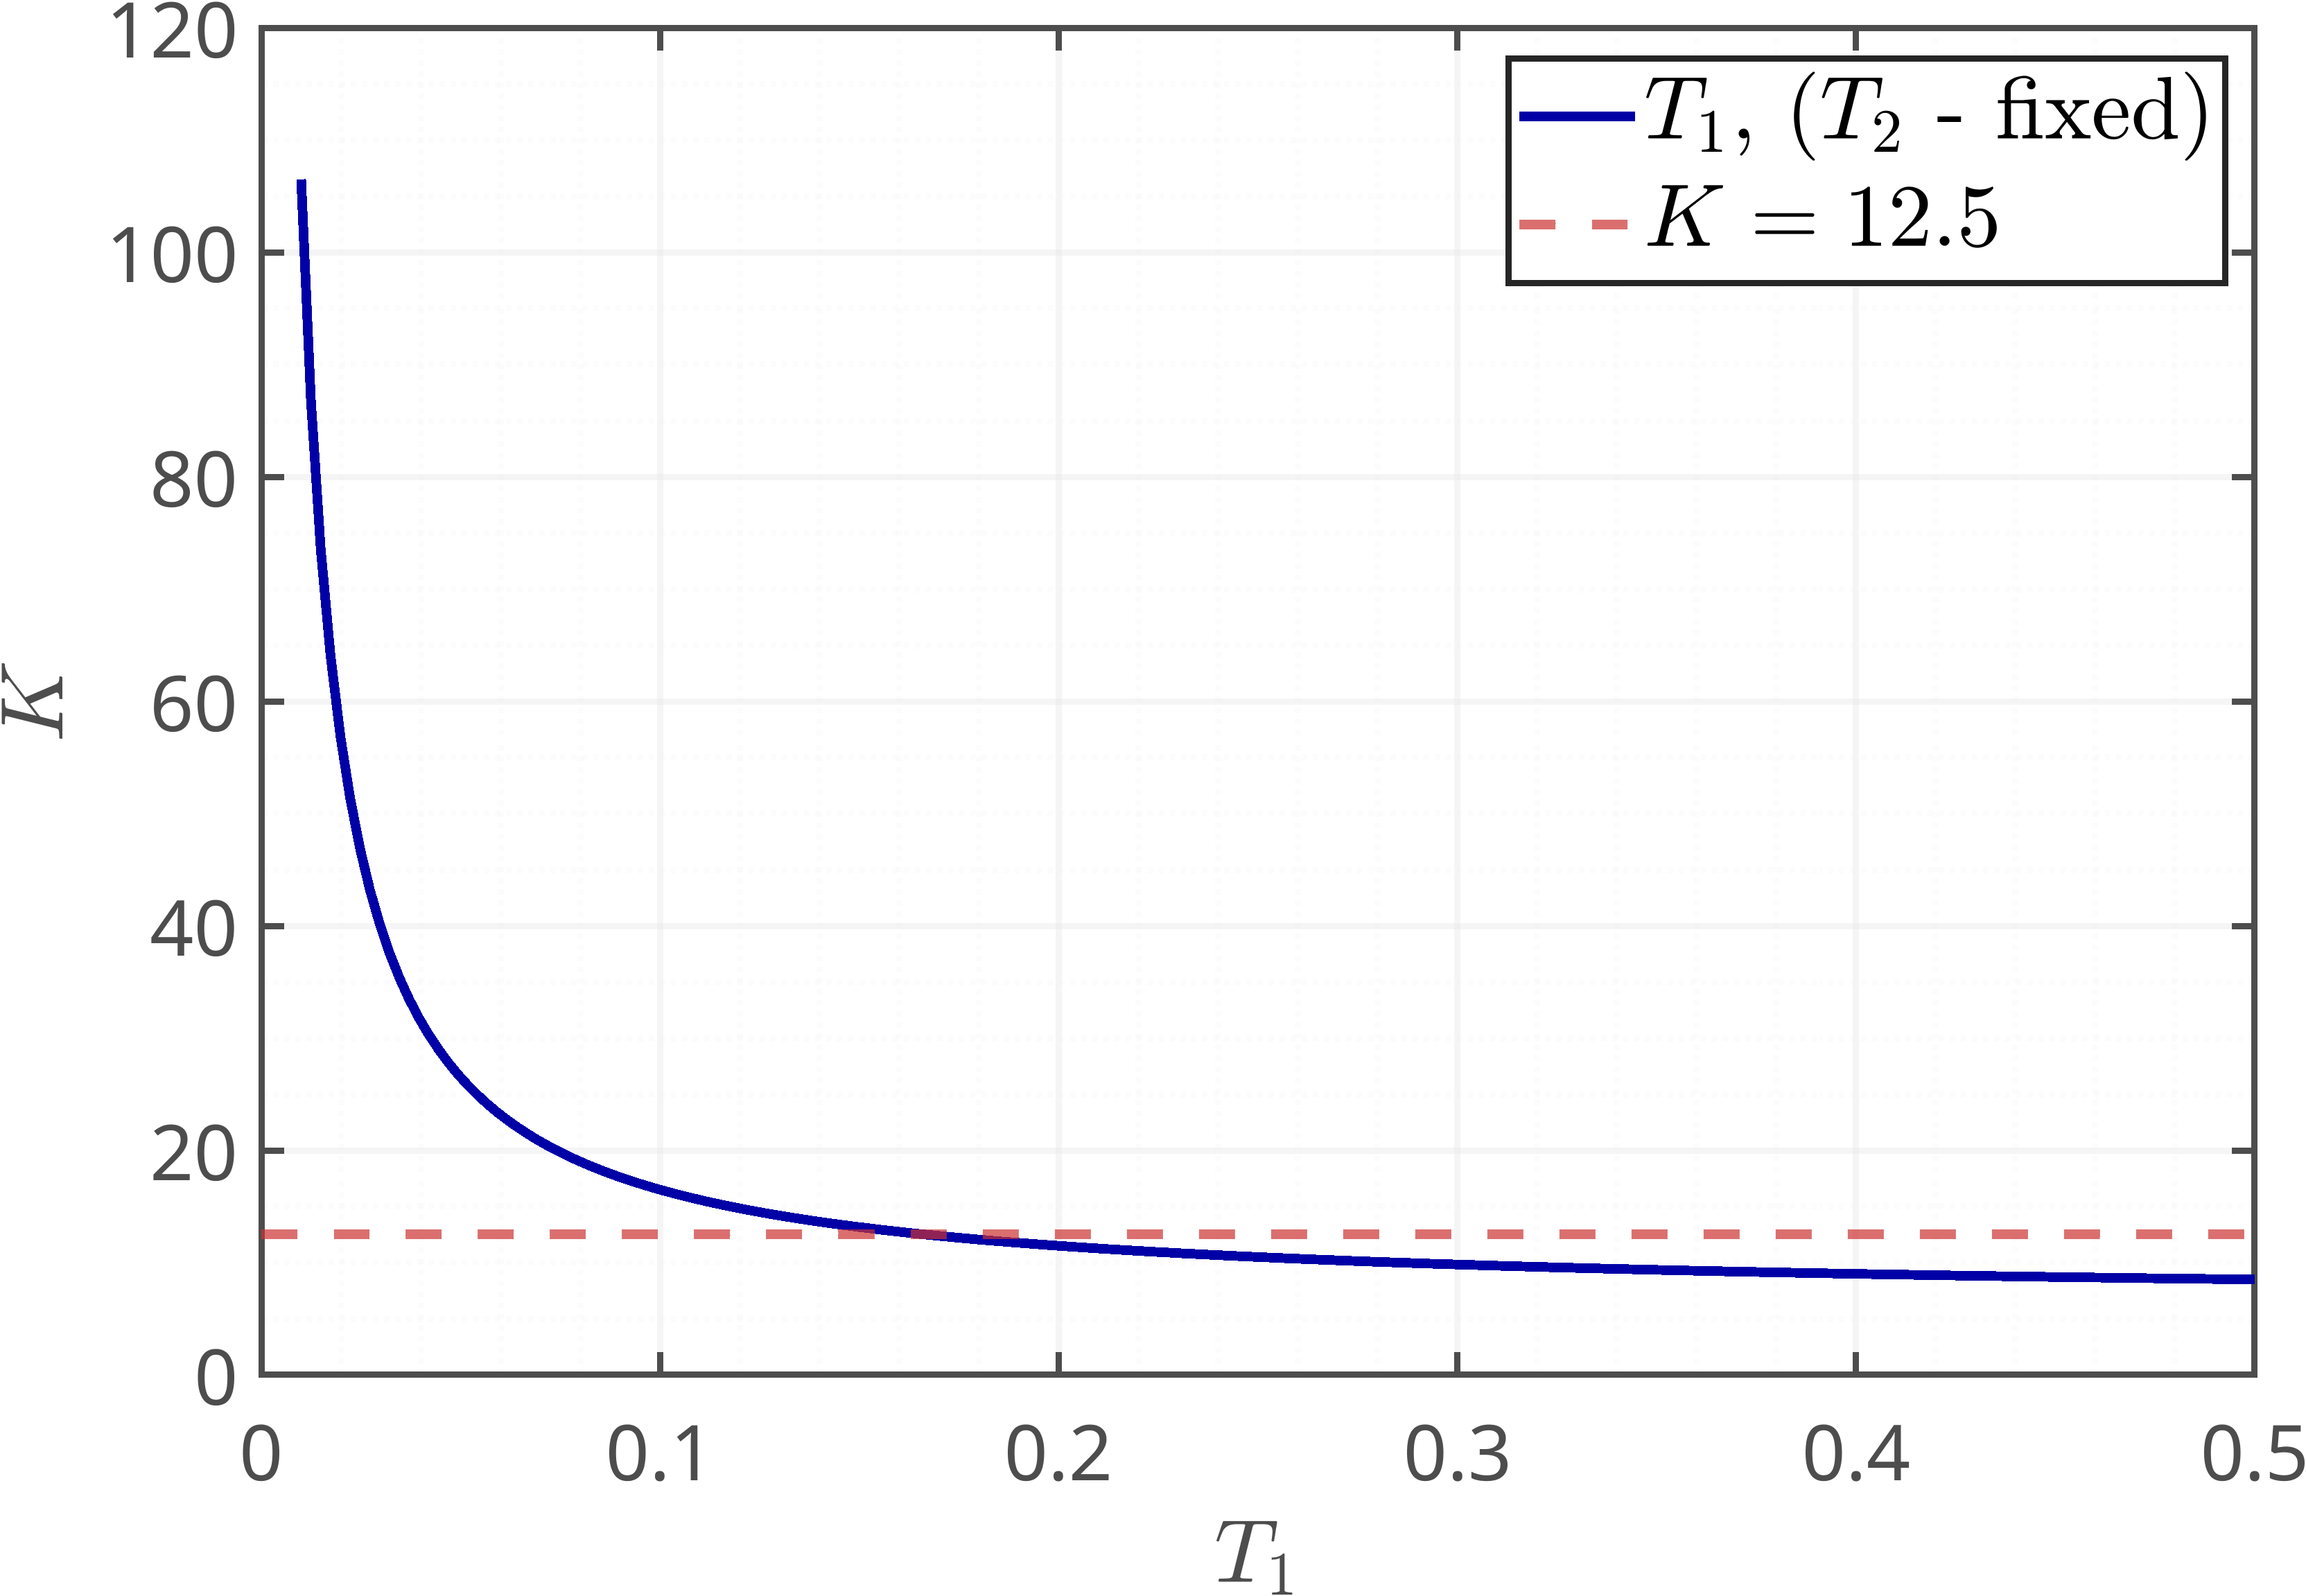
\includegraphics[width=\linewidth]{../images/task2/T1.png}
				\\[0.3em]
				\textbf{Граница устойчивости $K(T_1)$ при фиксированном $T_2$}
			\end{minipage}
			\hfill
			\begin{minipage}[b]{0.485\textwidth}
				\centering
				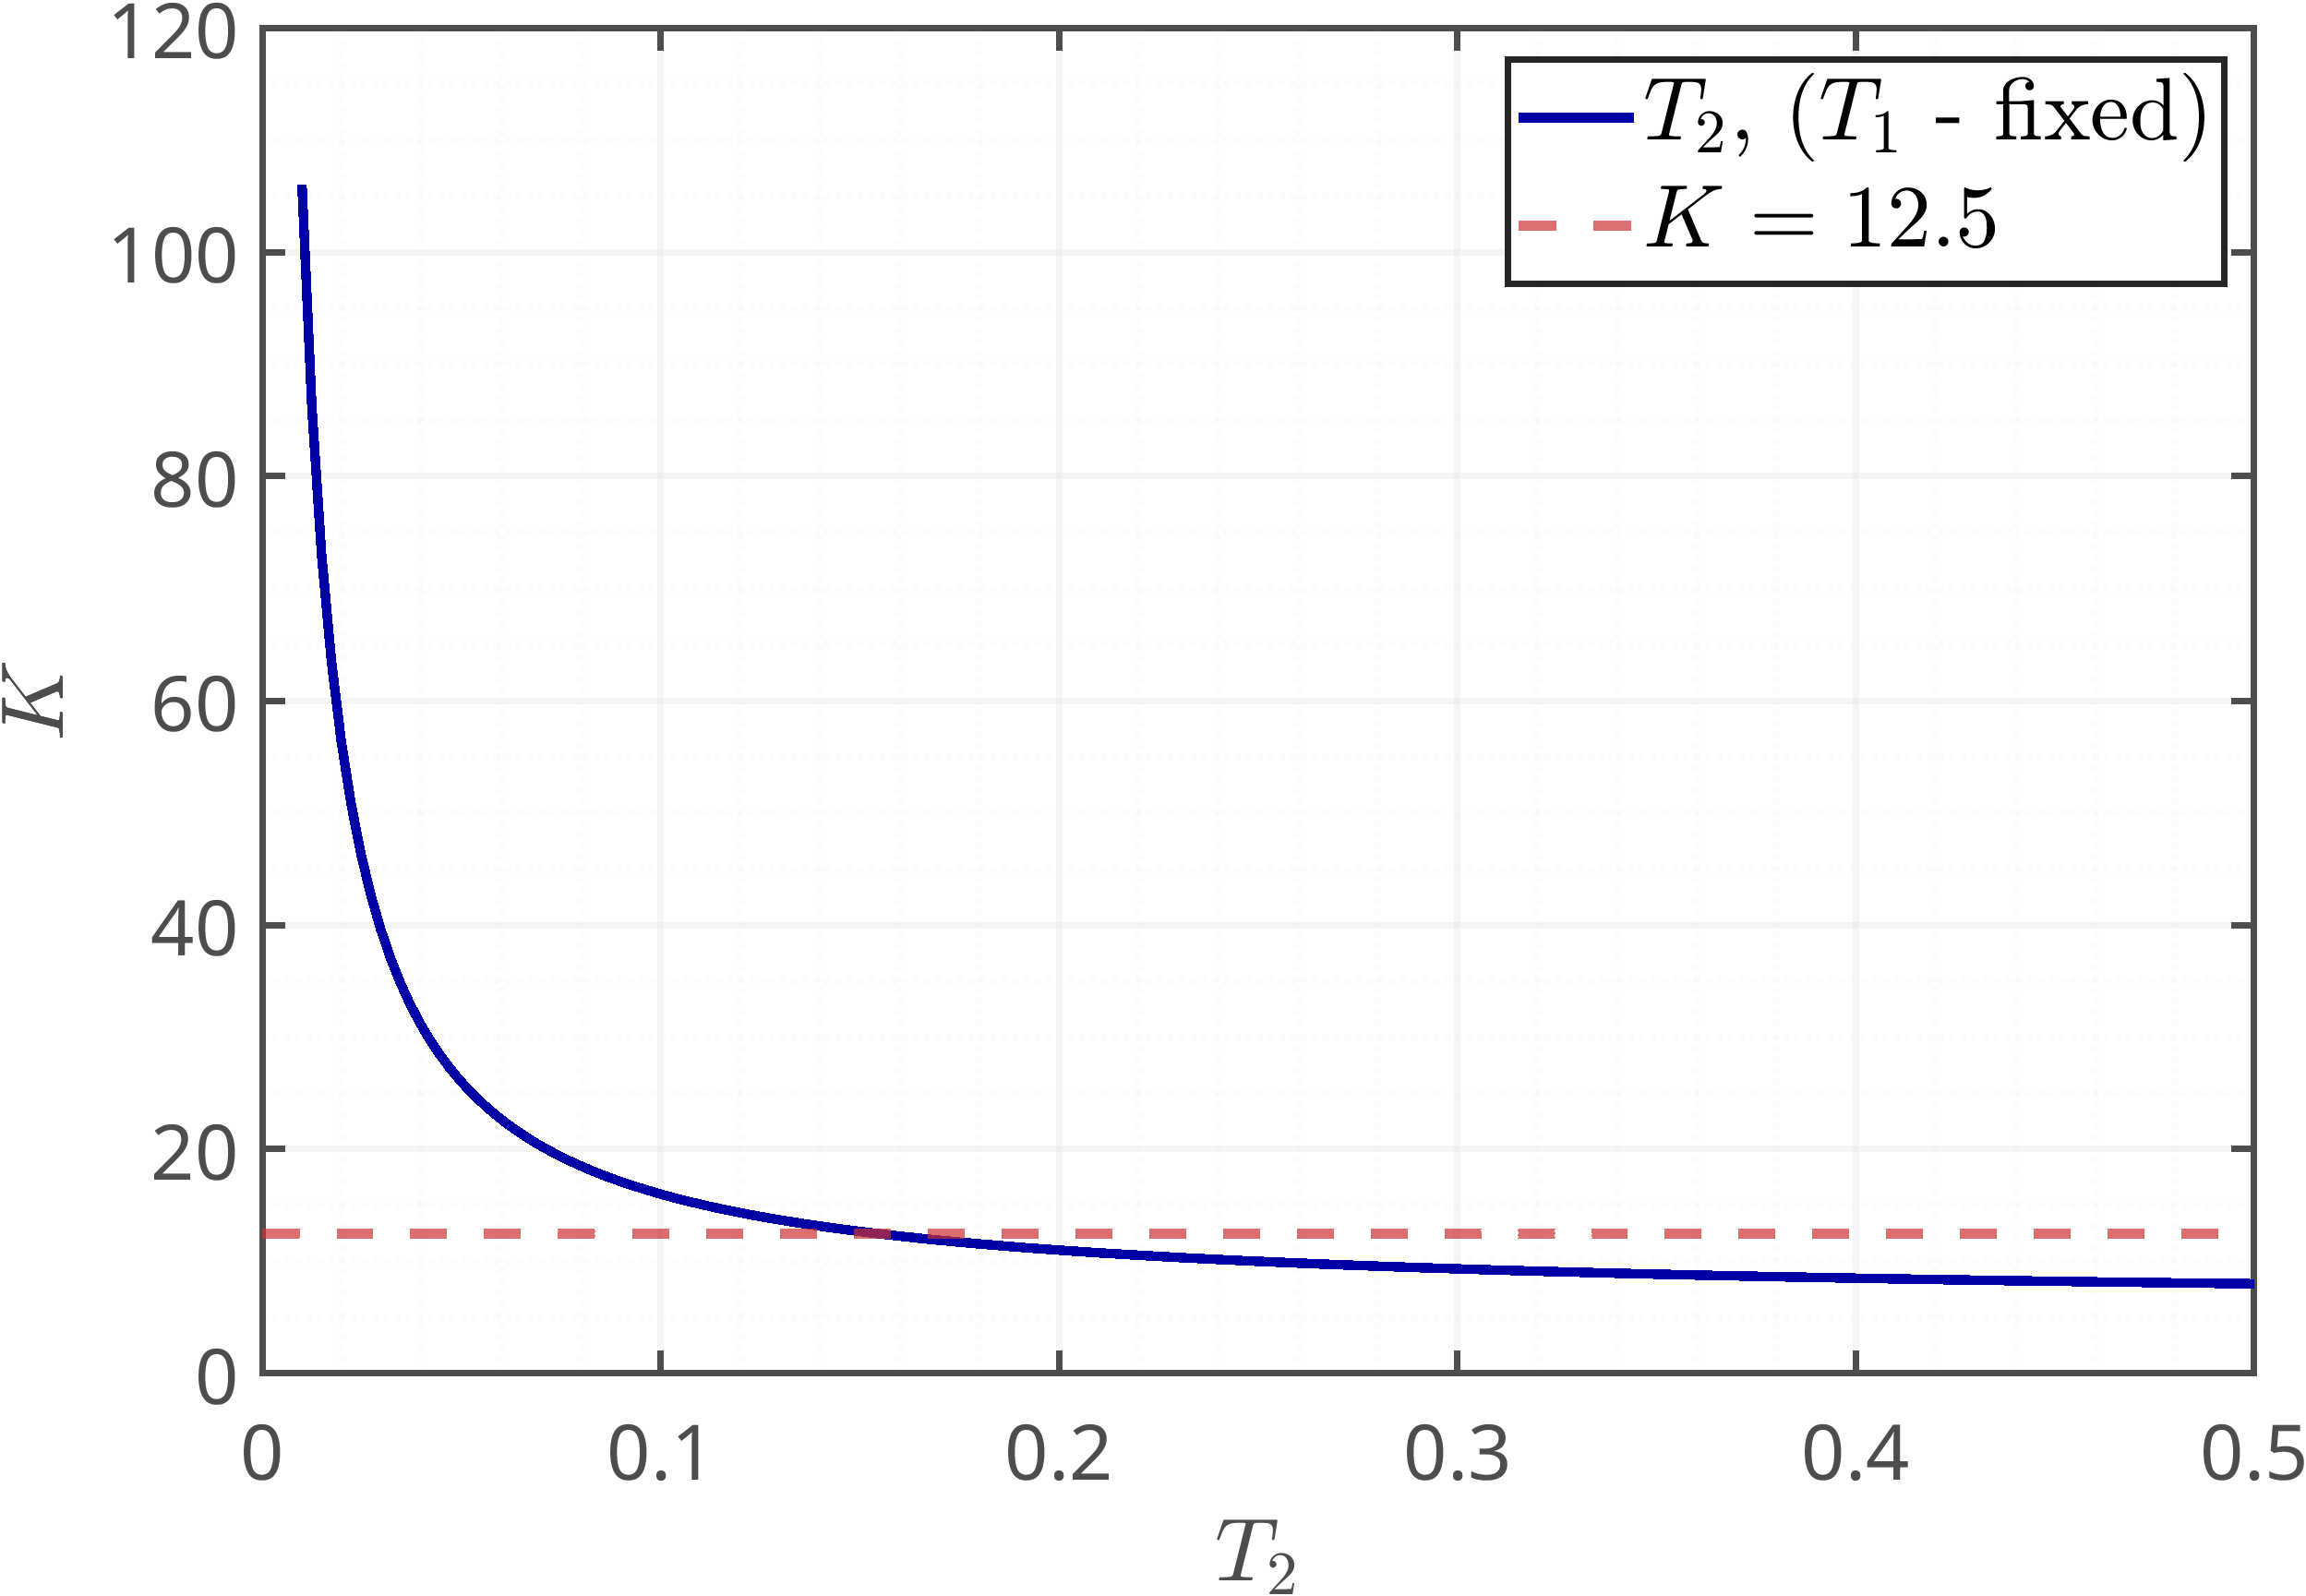
\includegraphics[width=\linewidth]{../images/task2/T2.png}
				\\[0.3em]
				\textbf{Граница устойчивости $K(T_2)$ при фиксированном $T_1$}
			\end{minipage}
			\caption{Графическое изображение границ устойчивости системы}
		\end{figure}
		
		\subsection{Графики выходов}
		
		На графиках показан выход системы.
		
		Рассмотрены три набора параметров:
		\begin{itemize}
			\item Устойчивая система: \(K=6\), \(T_1 = \dfrac{1}{6}\), \(T_2 = \dfrac{1}{6.5}\). Выход плавно приходит к постоянному значению.
			
		\item На границе устойчивости: \(K=12.5\), остальные параметры те же. Наблюдаются колебания постоянной амплитуды.
	
			\item Неустойчивая система: \(K=20\), \(T_1 = \dfrac{1}{6}\), \(T_2 = \dfrac{1}{6.5}\). Выход растёт с увеличением амплитуды.
		\end{itemize}
		
		Входное воздействие — единичная ступенчатая функция \(g(t) = 1(t)\).
		
		\begin{figure}[H]
			\centering
			
\includegraphics[width=1\textwidth]{../images/task2/y1.png}
			\caption{Устойчивая система}
		\end{figure}
		
		\begin{figure}[H]
			\centering
			
\includegraphics[width=1\textwidth]{../images/task2/y2.png}
			\caption{Система на границе устойчивости}
		\end{figure}
		
		\begin{figure}[H]
			\centering
			
\includegraphics[width=1\textwidth]{../images/task2/y3.png}
			\caption{Неустойчивая система}
		\end{figure}
		
		\textbf{Итог:} Для оценки устойчивости системы использовался критерий Гурвица. Я проверила условие, при котором все коэффициенты характеристического уравнения положительны и \(\Delta_2 > 0\). Результаты показали, что при \(K < 12.5\) система устойчива, при \(K = 12.5\) находится на границе устойчивости, а при \(K > 12.5\) — становится неустойчивой.
		
		\newpage
		\section{Задание.  Автономный генератор}
		
		В этом задании рассмотрю систему вида:
		\[
		\begin{cases}
			\dot{x} = A x \\
			g = Cx
		\end{cases}
		\]
		
		Требуется определить такие матрицы \( A \), \( C \) и начальное состояние \( x(0) \), чтобы свободный отклик системы совпадал с желаемым выходом:
		\[
		g_{\text{ж}}(t) = \cos(4t) + e^{-8t} \cos(5t)
		\]
		
		\subsection{Аналитические расчеты}
		
		Рассмотрю каждую составляющую выхода:
		
		\begin{itemize}
			\item \(\cos(4t)\) --- гармоническая составляющая, соответствующая комплексно-сопряжённым собственным значениям: \( \lambda_{1,2} = \pm 4i \).
			\item \(e^{-8t} \cos(5t)\) --- затухающая гармоническая составляющая, соответствующая собственным значениям: \( \lambda_{3,4} = -8 \pm 5i \).
		\end{itemize}
		
		Таким образом, матрица \( A \) должна иметь следующие собственные значения:
		\[
		\sigma(A) = \{ \pm 4i,\; -8 \pm 5i \}
		\]

		
		Построю матрицу \(A\) в жордановой форме:
		
		\[
		A =
		\begin{bmatrix}
			0 & 4 & 0 & 0 \\
			-4 & 0 & 0 & 0 \\
			0 & 0 & -8 & 5 \\
			0 & 0 & -5 & -8 \\
		\end{bmatrix}
		\]
		
		Общее решение линейной системы при нулевом входе:
		\[
		x(t) = e^{At} x(0), \quad g(t) = C x(t) = C e^{At} x(0)
		\]
				
		Запишу матричную экспоненту \( e^{At} \):
		\[
		e^{At} =
		\begin{bmatrix}
			\cos(4t) & \sin(4t) & 0 & 0 \\
			-\sin(4t) & \cos(4t) & 0 & 0 \\
			0 & 0 & e^{-8t} \cos(5t) & e^{-8t} \sin(5t) \\
			0 & 0 & -e^{-8t} \sin(5t) & e^{-8t} \cos(5t) \\
		\end{bmatrix}
		\]
		
		Вычислю выход системы по формуле:
		\[
		g(t) = C e^{At} x(0)
		\]
		
		Подставлю соответствующие выражения:
		
		\begin{align*}
			g(t) &= 
			\begin{bmatrix}
				c_1 & c_2 & c_3 & c_4
			\end{bmatrix}
			\cdot
			\begin{bmatrix}
				\cos(4t) & \sin(4t) & 0 & 0 \\
				-\sin(4t) & \cos(4t) & 0 & 0 \\
				0 & 0 & e^{-8t} \cos(5t) & e^{-8t} \sin(5t) \\
				0 & 0 & -e^{-8t} \sin(5t) & e^{-8t} \cos(5t)
			\end{bmatrix}
			\cdot
			\begin{bmatrix}
				a_1 \\ a_2 \\ a_3 \\ a_4
			\end{bmatrix}
			\\[1em]
			&=
			\begin{bmatrix}
				c_1 & c_2 & c_3 & c_4
			\end{bmatrix}
			\cdot
			\begin{bmatrix}
				a_1 \cos(4t) + a_2 \sin(4t) \\
				-a_1 \sin(4t) + a_2 \cos(4t) \\
				a_3 e^{-8t} \cos(5t) + a_4 e^{-8t} \sin(5t) \\
				-a_3 e^{-8t} \sin(5t) + a_4 e^{-8t} \cos(5t)
			\end{bmatrix}
			\\[1em]
			&=
			\left( a_1 c_1 + a_2 c_2 \right) \cos(4t)
			+ \left( a_2 c_1 - a_1 c_2 \right) \sin(4t)
		 + e^{-8t} \left[
			\left( a_3 c_3 + a_4 c_4 \right) \cos(5t)
			+ \left( a_4 c_3 - a_3 c_4 \right) \sin(5t)
			\right]
		\end{align*}
		
		Получу:	
		\[
		g(t) = 
		\underbrace{(a_1 c_1 + a_2 c_2)}_{\text{коэф. при } \cos(4t)} \cos(4t)
		+ 
		\underbrace{(a_2 c_1 - a_1 c_2)}_{\text{коэф. при } \sin(4t)} \sin(4t)
		+ e^{-8t} \left[
		\underbrace{(a_3 c_3 + a_4 c_4)}_{\text{коэф. при } \cos(5t)} \cos(5t)
		+ 
		\underbrace{(a_4 c_3 - a_3 c_4)}_{\text{коэф. при } \sin(5t)} \sin(5t)
		\right]
		\]
		
		
		Теперь подберу коэффициенты для того, чтобы получить желаемый выход:
		\[
		g_{\text{ж}}(t) = \cos(4t) + e^{-8t} \cos(5t)
		\]
		
		Чтобы \(g(t) \equiv g_\text{ж}(t)\) , должны совпадать коэффициенты при соответствующих гармонических функциях.
		
		Сравнивая коэффициенты, получаю систему:
		
		\[
		\begin{cases}
			a_1 c_1 + a_2 c_2 = 1 \\
			a_2 c_1 - a_1 c_2 = 0 \\
			a_3 c_3 + a_4 c_4 = 1 \\
			a_4 c_3 - a_3 c_4 = 0 \\
		\end{cases}
		\]
		
		Чтобы упростить решение, выберу:
		\[
		a_2 = 0, \quad a_4 = 0
		\]
		
		Тогда первые два уравнения примут вид:
		\[
		\begin{cases}
			a_1 c_1 = 1 \\
			- a_1 c_2 = 0
		\end{cases}
		\quad \Rightarrow \quad
		\begin{cases}
			a_1 c_1 = 1 \\
			c_2 = 0
		\end{cases}
		\]
		
		А последние два уравнения:
		\[
		\begin{cases}
			a_3 c_3 = 1 \\
			- a_3 c_4 = 0
		\end{cases}
		\quad \Rightarrow \quad
		\begin{cases}
			a_3 c_3 = 1 \\
			c_4 = 0
		\end{cases}
		\]
		
		Ещё упрощу решение, положу: \(a_1 = 1\) и \(a_3 = 1\). Тогда получу:
		\[
		c_1 = 1, \quad c_2 = 0, \quad c_3 = 1, \quad c_4 = 0
		\]
		
		В итоге получаю:
		
		\[
		A =
		\begin{bmatrix}
			0 & 4 & 0 & 0 \\
			-4 & 0 & 0 & 0 \\
			0 & 0 & -8 & 5 \\
			0 & 0 & -5 & -8 \\
		\end{bmatrix}, \quad
		x(0) =
		\begin{bmatrix}
			1 \\
			0 \\
			1 \\
			0 \\
		\end{bmatrix}, \quad
		C =
		\begin{bmatrix}
			1 & 0 & 1 & 0
		\end{bmatrix}
		\]
		
		\subsection{График сигналов}
		
		Построю график выходного сигнала системы, вычесленного через матрицы состояния и заданного желаемого выхода системы.
		
		\begin{figure}[H]
			\centering
			
\includegraphics[width=1\textwidth]{../images/task3/g.png}
			\caption{График \(g(t)\) и \(g_\text{ж}(t)\)}
		\end{figure}
		
		\subsection{График ошибки}
		
		\begin{figure}[H]
			\centering
			
\includegraphics[width=1\textwidth]{../images/task3/e.png}
			\caption{График \(e = g_\text{ж}(t) - g(t)\)}
		\end{figure}
		
		\textbf{Итог: } Автономный генератор воспроизводит желаемый сигнал.
		
		\newpage
		\section{Вывод}
		

\par
	В лабораторной работе я исследовала линейные динамические системы различного порядка.
	Для системы второго порядка я показала зависимость переходного процесса от корней характеристического уравнения. В системе третьего порядка я нашла границу устойчивости и изучила влияние параметров на устойчивость. Для автономного генератора я подобрала параметры, обеспечивающие генерацию нужного сигнала.

\end{document}